\documentclass{article}

\usepackage{amsmath}
\usepackage{amssymb}
\usepackage{amsfonts}
\usepackage[margin=1in]{geometry}
\usepackage{pgfplots}
\pgfplotsset{compat=1.3}
\usepgfplotslibrary{colormaps}

\begin{document}
    
\section*{Introduction}

The purpose of this document is to explore the trade-off between the size of an antialising region
and the approximate accuracy of an integral of a state function $f(\mathbf{x}, t)$ which we assume
to be continuously differentiable in $(\mathbf{x}, t)$.
\\
\\
In Smoothlife, we discretize a domain with periodic boundaries using rectangles of some prescribed width and height. To this end, we are given the value of a state function in each cell, i.e. an approximation of some state function at the midpoint of each cell. In practice, this means that we can take the circular (and annular) regions of integration to be centered at the midpoint of any given cell in the grid.
    
\section{Motivation: Weight functions in 1D}

We begin by looking at a 1D analogue of the operations we perform in Smoothlife, specifically a function defined on $D := [0, r]$ for some $r > 0$. In addition, define an antialiasing parameter $b > 0$. Then we are tasked, for some "smooth-enough" state function $f : \mathbb{R} \rightarrow [0, \infty)$
\[
    \int_0^r f(x) \: dx
\]

\noindent
In Smoothlife, however, we extend $D$ to $D_b = [0, r + b/2]$. In addition, let
\[
    \omega_b(x)=
    \begin{cases}
        1, & 0 \leq x \leq r - \dfrac{b}{2} \\
        \dfrac{r + b/2 - x}{b} & x > r - \dfrac{b}{2}
    \end{cases}
\]

\begin{figure}[h]
    \centering
    \begin{tikzpicture}
        \begin{axis}[
            title={Weight Function},
            xlabel={$x$},
            ylabel={$\omega_b(x)$},
            xticklabel=\empty,   
        ]
            % density of Normal distribution:
            \addplot [
                red,
                domain=0:4,
                samples=5
            ]{and(\x>=0, \x<=3) * (1) +
                and(\x>3, \x<=4) * (4 - \x)};
            
            
            \addplot[dashed, black] coordinates {(2.75,0) (2.75,1)} node[below left]{\footnotesize $x_i$};
            
            \addplot[dashed, black] coordinates {(3.5,0) (3.5,1)} node[below left]{\footnotesize $x_{i+1}$};
        \end{axis}
    \end{tikzpicture}
\end{figure}

\noindent
Then the integral approximation to $f$ on $D$ is given by
\[
    \int_{D_b} f(x) \omega_b(x) \: dx
\]

\noindent
This is motivated by the need to approximate the circular nature of the domain using an antialiasing region of width $b > 0$.
\\
\\
We can then define the error on $D_b$ as
\[
    E_b := \int_{D_b} f(x) (1 - \omega_b(x)) \: dx
    =
    \int_{r-b/2}^{r+b/2} f(x)
    \dfrac{r + b/2 - x}{b} \: dx,
\]

\noindent
which shows that the error is amplified in the antialiasing region. This formulation introduces a couple of issues, one of which is that we are approximating the integral of a nonsmooth integrand (really, an integrand with a nonsmooth weight) using a quadrature rule (the midpoint rule) where we cannot rely on the smoothness of the integrand.
\\
\\
What we hope to show is that we need to find a trade-off between the discretization and the size of the anti-aliasing region. Our conjectures are as follows:

\begin{enumerate}
    \item If a node of the partition of $D_b$ falls on $x = r$, then the global order of approximation could decrease the order of convergence from quadratic to linear.
    \item If $b \in (x_j, x_{j+1})$ for some $j = 0, 1, ..., n-1$, then the error in the approximation will be a function of the magnitude of $b$ and and the distance to $x = r$.    
\end{enumerate}

\noindent
In the next sections, we will explore the above conjectures in the case $f(x) \equiv 1$, saving the general case for later.

\newpage

\section{The case of $f(x) \equiv 1$}
\subsection{A subinterval containing $x = r - b/2$}

Consider a partition $P_n$ of $D_b$ with $0 = x_0 < x_1 < \cdots < x_n = r + b/2$, and suppose there is an integer $j$, $0 \leq j \leq n - 1$ such that $r \in (x_j, x_{j+1})$. In addition, let $I_i = [x_i, x_{i+1}]$ for $i = 0, 1, \ldots, n-1$, let $\Delta x_i = x_{i+1} - x_i$ for $i = 0, 1, \ldots, n-1$, and let $s = \dfrac{r - b/2 - x_j}{\Delta x_j}$. Then we know that the exact integral under this region is given by
\[
    \begin{array}{rcl}
    A_j &=& \displaystyle
            \int_{x_j}^{x_{j+1}} \omega_b(x) \: dx \\
        & &	\\
        &=& \displaystyle
            \int_{x_j}^{r-b/2} 1 \: dx +
            \int_{r-b/2}^{x_{j+1}} \frac{r+b/2-x}{b} \: dx \\
        & &	\\
        &=& \displaystyle
            (r - b/2 - x_j) +
            \frac{1}{2}
            \left( 1 + \dfrac{r + b/2 - x_{j+1}}{b} \right)
            (x_{j+1} - (r - b/2)) \\
        & &	\\
        &=& \displaystyle
            s\Delta x_j +
            \frac{1}{2}
            \left( 1 + \dfrac{r + b/2 - x_{j+1}}{b} \right)
            (1 - s) \Delta x_j \\
        & &	\\
        &=& \displaystyle
            s\Delta x_j +
            \frac{1}{2}
            \left(
                \frac{r + b/2 - (r - b/2)}{b} +
                \frac{r + b/2 - x_{j+1}}{b}
            \right)
            (1 - s) \Delta x_j \\
        & &	\\
        &=& \displaystyle
            s\Delta x_j +
            \left(
                \frac{
                    r + b/2 -
                    \frac{x_{j+1} + (r - b/2)}{2}
                }{b}
            \right)
            (1 - s) \Delta x_j \\
    \end{array}
\]

\noindent
Due to the equivalence of the midpoint and trapezoidal sums for affine functions, we can write the area under the trapezoidal portion of $\omega_b(x)$ on $(r - b/2, x_{j+1})$ as a midpoint sum (see above). We will be utilizing this later to show the error approximation when the midpoint of the interval $I_j$ is greater than $r - b/2$.
\\
\\
For the remaining subintervals forming $P_n$, the quadrature will be exact due to the midpoint rule being exact for linear functions, meaning the interval $I_j$ will control the error of the approximation. Now let $M_j$ be the midpoint approximation to the desired integral on interval $I_j$, $m_j = \dfrac{x_j + x_{j+1}}{2}$, and $\Delta x_j := x_{j+1} - x_j$. Then we have the following:
\[
    M_j := 
    \begin{cases}
        \Delta x_j, & m_j \leq r - b/2 \\
        \dfrac{r + b/2 - m_j}{b} \Delta x_j, & m_j > r - b/2
    \end{cases}
\]

\noindent
By construction, $E_j = 0$ when $x_j = r - b/2$ or $x_{j+1} = r - b/2$ since the midpoint rule is exact strictly on the constant or nonconstant regions of $\omega_b(x)$.
\\
\\
Now let $E_j := A_j - M_j$. On the interval $I_j$, we have
\[
    \begin{array}{rcl}
    E_j &=& \displaystyle
            \frac{1}{2} \left[
                1 + \dfrac{r + b/2 - x_{j+1}}{b}
            \right] (x_{j+1} - (r - b/2)) -
            (x_{j+1} - (r-b/2)) \\
        & &	\\
        &=& \displaystyle
            \frac{1}{2} \left[
            1 + \dfrac{r + b/2 - x_{j+1}}{b}
            \right] (1 - s)\Delta x_j -
            (1 - s)\Delta x_j \\
        & &	\\
        &=& \displaystyle
            \frac{1}{2} \left[
                -1 + \dfrac{r + b/2 - x_{j+1}}{b}
            \right] (1 - s)\Delta x_j \\
        & &	\\
        &=& \displaystyle
            \frac{1}{2} \left[
            -\frac{r + b/2 - (r - b/2)}{b}
            +
            \frac{r + b/2 - x_{j+1}}{b}
            \right] (1 - s)\Delta x_j \\
        & &	\\
        &=& \displaystyle
            \frac{1}{2} \left[
                \frac{(r - b/2) - (r + b/2)}{b}
                +
                \frac{r + b/2 - x_{j+1}}{b}
            \right] (1 - s)\Delta x_j \\
        & &	\\
        &=& \displaystyle
            \frac{1}{2} \left[
                \frac{r - b/2 - x_{j+1}}{b}
            \right] (1 - s)\Delta x_j \\
        & &	\\
        &=& \displaystyle
            -\frac{1}{2} \left[
                \frac{x_{j+1} - (r - b/2)}{b}
            \right] (1 - s)\Delta x_j \\
        & &	\\
        &=& \displaystyle
            -\frac{1}{2b}(1 - s)^2\Delta x_j^2 \\
    \end{array}
\]

\noindent
when $m_j \leq r - b/2$ or $s \geq 1/2$. Indeed, $E_j$ can be interpreted as the signed over-estimation error that comes from approximating the area under $\omega_b(x)$ on $(r - b/2, x_{j+1}]$ by use of the midpoint rule on $I_j$.
\\
\\
Now suppose that $m_j > r - b/2$ ($s < 1/2$), and recall that the midpoint rule and the trapezoidal rule are equivalent for affine functions. In addition, note that we can split the midpoint rule using some algebra:
\[
    \begin{array}{rcl}
        M_j &=& \displaystyle
                \left[
                    \frac{r + b/2 -
                        \frac{x_{j+1}+x_j}{2}
                    }{b}
                \right]
                (1 - s)\Delta x_j
                +
                \left[
                    \frac{r + b/2 -
                        \frac{x_{j+1}+x_j}{2}
                    }{b}
                \right]
                s\Delta x_j \\
    \end{array}
\]

\noindent
The purpose of this is to make easier the computation of the overall error by grouping terms involve $(1 - s) \Delta x_j$ and $s\Delta x_j$. To proceed, let's focus on the term attached to $(1 - s)\Delta x_j$. Then that portion of $E_j = A_j - M_j$ simplifies to 

\[
\begin{array}{rcl}
    E_j &=& \displaystyle
            \left(
            \frac{
                r + b/2 -
                \frac{x_{j+1} + (r - b/2)}{2}
            }{b}
            -
            \frac{
                r + b/2 -
                \frac{x_{j+1} + x_j}{2}
            }{b}
            \right) (1 - s) \Delta x_j \\
        & & \\
        &=& \displaystyle
            \left(
            \frac{
                - \frac{x_{j+1} - (r - b/2)}{2}
                + \frac{x_{j+1} + x_j}{2}
            }{b}
            \right) (1 - s) \Delta x_j \\
        & & \\
        &=& \displaystyle
            \frac{1}{2}
            \left(
                \frac{
                    - x_{j+1} - (r - b/2)
                    + x_{j+1} + x_j
                }{b}
            \right) (1 - s) \Delta x_j \\
        & & \\
        &=& \displaystyle
            \frac{1}{2}
            \left(
                \frac{
                    -(r - b/2) + x_j
                }{b}
            \right) (1 - s) \Delta x_j \\
        & & \\
        &=& \displaystyle
            -\frac{1}{2}
            \left(
                \frac{
                    r - b/2 - x_j
                }{b}
            \right) (1 - s) \Delta x_j \\
        & & \\
        &=& \displaystyle
            -\frac{1}{2b}
            s\Delta x_j (1 - s) \Delta x_j \\
            & & \\
            &=& \displaystyle
            -\frac{1}{2b} s(1 - s) \Delta x_j^2
\end{array}
\]

\noindent
Next we tackle the $s\Delta x_j$ term. 

\[
\begin{array}{rcl}
    E_j &=& \displaystyle
            \left(
                1
                -
                \frac{
                    r + b/2 -
                    \frac{x_{j+1} + x_j}{2}
                }{b}
            \right) s \Delta x_j \\
        & & \\
        &=& \displaystyle
            \left(
                \frac{
                    r + b/2 - (r - b/2)
                    -
                    (r + b/2)
                    +
                    \frac{x_{j+1} + x_j}{2}
                }{b}
            \right) s \Delta x_j \\
        & & \\
        &=& \displaystyle
        \frac{1}{2}
        \left(
            \frac{
                -2(r - b/2)
                +
                x_{j+1} + x_j
            }{b}
        \right) s \Delta x_j \\
        & & \\
        &=& \displaystyle
        -\frac{1}{2}
        \left(
            \frac{
                r - b/2 - x_j
            }{b}
        \right) s \Delta x_j
        +
        \frac{1}{2}
        \left(
            \frac{
                x_{j+1} - (r - b/2)
            }{b}
        \right) s \Delta x_j \\
        & & \\
        &=& \displaystyle
        -\frac{1}{2b} s^2 \Delta x_j^2
        +
        \frac{1}{2b} s(1 - s) \Delta x_j^2 \\
\end{array}
\]

\noindent
Combining both results yields
\[
    E_j = -\frac{1}{2b} s^2 \Delta x_j^2
\]

\noindent
for $m_j > r - b/2$. Combining these results yields
\[
    E_j =
    \begin{cases}
        -\dfrac{1}{2b} s^2 \Delta x_j^2, & s < 1/2
        \\ \\
        -\dfrac{1}{2b} (1-s)^2 \Delta x_j^2, & s \geq 1/2
    \end{cases}
\]

\newpage

\subsection{A partition that extends beyond the support of $\omega_b(x)$}

In practice, the domains over which we integrate in smooth life will have to contend with a rectangular grid where some portions of the curves do not perfectly meet at a convenient boundary of a cell. This will especially be common in the case where we have a very fine grid of cells. This leaves us with a few options:

\begin{enumerate}
    \item Ignore a cell if the midpoint is outside of the domain of integration, even if there is nontrivial overlap of the cell and the interior of the region of integration.
        \begin{itemize}
            \item Otherwise, compute the overlap of the interval and deal with the overestimate of the value of the integral.
        \end{itemize}
    
    \item Use Green's theorem to find the centroid of the region where there is overlap with the cell.
        \begin{itemize}
            \item In $\mathbb{R}^2$, we'll rely on Green's theorem.  
        \end{itemize}
\end{enumerate}

\noindent
We'll start with the first scenario below, and then take a look at using Green's theorem in 2D. In practice, these calculations just have to be done once on initialization, and then can be re-used since in practice we're just shifting in the values of the state function f.

\subsubsection{The 1D Case}

In the case of a 1-dimensional function, suppose we have a partition where the intersection $I_{n-1} = [x_{n-1},x_n]$ and $D_b = [0, r+b/2]$ is non-empty, but for which $I_{n-1} \cap D_b \subsetneq I_{n-1}$. Furthermore, let

\[
    t = \frac{r + b/2 - x_{n-1}}{\Delta x_{n-1}}
\]

\noindent
Then the exact area of the triangular sliver on $[x_{n-1}, r+b/2]$ is given by

\[
\begin{array}{rcl}
    A_{n-1} &=& \displaystyle
                \frac{1}{2}
                t \Delta x_{n-1}
                \left(
                    \frac{r + b/2 - x_{n-1}}{b}
                \right)
                \\
            & &	\\
            &=& \displaystyle
                \frac{1}{2b}
                t^2 \Delta x_{n-1}^2
                \\
\end{array}
\]

\noindent
The approximation using the midpoint rule on $I_{n-1}$ is as follows:

\[
\begin{array}{rcl}
    M_{n-1} &=& \displaystyle
                \Delta x_{n-1}
                \frac{r + \frac{b}{2} - \frac{x_{n-1} + x_n}{2}}{b}
                \\
            & &	\\
            &=& \displaystyle
                \frac{1}{2b}
                \Delta x_{n-1}
                \left(
                2r + b - x_{n-1} - x_n
                \right)
                \\
            & &	\\
            &=& \displaystyle
                \frac{1}{2b}
                \Delta x_{n-1}
                \left(
                r + \frac{b}{2} - x_{n-1}
                +
                r + \frac{b}{2} - x_n
                \right)
                \\
            & &	\\
            &=& \displaystyle
                \frac{1}{2b}
                \Delta x_{n-1}
                \left(
                    r + \frac{b}{2} - x_{n-1}
                    -
                    \left(
                        x_n
                        -
                        \left(
                            r + \frac{b}{2}
                        \right)
                    \right)
                \right)
                \\
            & &	\\
            &=& \displaystyle
                \frac{1}{2b}
                \Delta x_{n-1}
                (
                    t \Delta x_{n-1}
                    -
                    (1 - t) \Delta x_{n-1}
                )
                \\
            & &	\\
            &=& \displaystyle
                \frac{1}{2b}
                (2t - 1)\Delta x_{n-1}^2
                \\
\end{array}
\]

\noindent
provided

\[
    \frac{x_{n-1} + x_n}{2} \leq r + \frac{b}{2}
    \iff
    \frac{x_n - x_{n-1}}{2} \leq r + \frac{b}{2} - x_{n-1}
    \iff
    \frac{\Delta x_{n-1}}{2} \leq t \Delta x_{n-1}
    \iff
    t \geq \frac{1}{2}.
\]

\noindent
In the case that $0 < t < \frac{1}{2}$ or $frac{x_{n-1} + x_n}{2} > r + \frac{b}{2}$, the integrand $\omega_b(x) = 0$ at midpoint sampled in $I_{n-1}$, and so $M_{n-1} = 0$. Altogether, we see that

\[
    M_{n-1}
    =
    \begin{cases}
        0, & 0 < t < \dfrac{1}{2}
        \\
        \\
        \dfrac{1}{2b}
        (2t - 1)
        \Delta x_{n-1}^2, & \dfrac{1}{2} \leq t < 1
    \end{cases}
\]

\noindent
with the error given by
\[
    E_{n-1}
    =
    \begin{cases}
        \dfrac{1}{2b}
        t^2
        \Delta x_{n-1}^2, & 0 < t < \dfrac{1}{2}
        \\
        \\
        \dfrac{1}{2b}
        (1 - t)^2
        \Delta x_{n-1}^2, & \dfrac{1}{2} \leq t < 1
    \end{cases}
\]

\subsection{Collecting Error Terms}

For the partition $P$, we have that the total nonzero errors can be collected as $E_P = E_j + E_{n-1}$:

\[
    E_P
    =
    \begin{cases}
        \dfrac{1}{2b}
        t^2
        \Delta x_{n-1}^2
        -
        \dfrac{1}{2b}
        s^2 \Delta x_j^2, & 0 < s < \dfrac{1}{2}, \: 0 < t < \dfrac{1}{2}
        \\
        \\
        \dfrac{1}{2b}
        t^2
        \Delta x_{n-1}^2
        -
        \dfrac{1}{2b}
        (1-s)^2 \Delta x_j^2, & \dfrac{1}{2} \leq s < 1, \: 0 < t < \dfrac{1}{2}
        \\
        \\
        \dfrac{1}{2b}
        (1 - t)^2
        \Delta x_{n-1}^2
        -
        \dfrac{1}{2b}
        s^2 \Delta x_j^2, & 0 < s < \dfrac{1}{2}, \: \dfrac{1}{2} \leq t < 1
        \\
        \\
        \dfrac{1}{2b}
        (1 - t)^2
        \Delta x_{n-1}^2
        -
        \dfrac{1}{2b}
        (1-s)^2 \Delta x_j^2, & \dfrac{1}{2} \leq s < 1, \: \dfrac{1}{2} \leq t < 1
    \end{cases}
\]

\noindent
In the 2D case, we typically take the partition to be uniform, and we can assume that to be the case here. This means $\Delta x_i = h_P > 0$ for all $i = 0, 1, \ldots, n-1$. Thus

\[
E_P
=
\begin{cases}
    \dfrac{1}{2b}
    (t^2 - s^2)
    h_P^2, & 0 < s < \dfrac{1}{2}, \: 0 < t < \dfrac{1}{2}
    \\
    \\
    \dfrac{1}{2b}
    (t^2 - (1 - s)^2)
    h_P^2, & \dfrac{1}{2} \leq s < 1, \: 0 < t < \dfrac{1}{2}
    \\
    \\
    \dfrac{1}{2b}
    ((1 - t)^2 - s^2)
    h_P^2, & 0 < s < \dfrac{1}{2}, \: \dfrac{1}{2} \leq t < 1
    \\
    \\
    \dfrac{1}{2b}
    ((1 - t)^2 - (1 - s)^2)
    h_P^2, & \dfrac{1}{2} \leq s < 1, \: \dfrac{1}{2} \leq t < 1
\end{cases}
\]

\noindent
Going further, we can plot $E_P$ as a function of $(s,t)$ on the unit square $[0,1]^2 \subset \mathbb{R}^2$, see Figure ~\ref{fig:midpterr}.

\newpage

\begin{figure}[h]
    \centering
    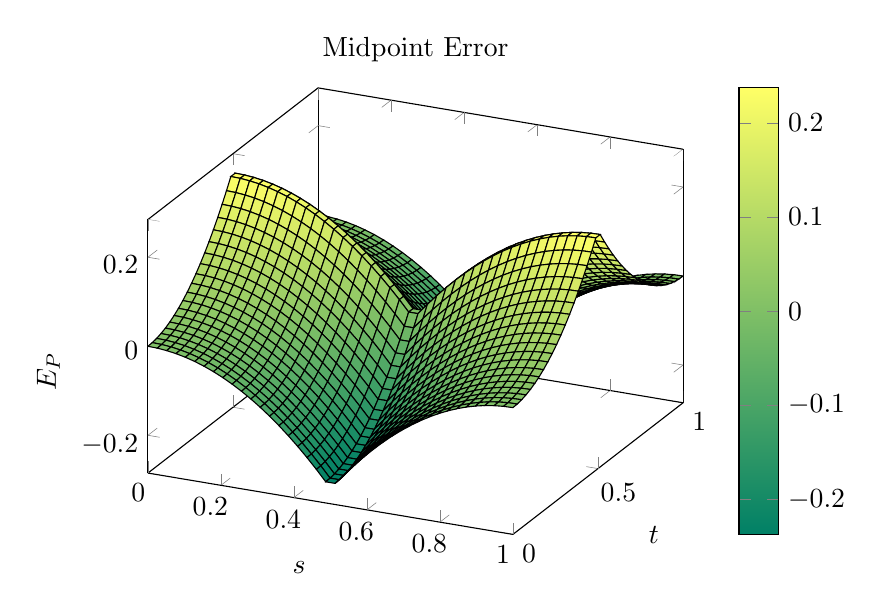
\begin{tikzpicture}
        \begin{axis}[colorbar, colormap/summer, xlabel=$s$,
            ylabel=$t$, zlabel=$E_P$, title=Midpoint Error]
            \addplot3 [
                surf,
                %shader=flat,
                samples=40,
                faceted color=black,
                domain=0:1,
                y domain=0:1
            ] {(y^2 - x^2) * and(x < 0.5, y < 0.5)
               +
               (y^2 - (1-x)^2) * and(x >= 0.5, y < 0.5)
               +
               ((1-y)^2 - x^2) * and(x < 0.5, y >= 0.5)
               +
               ((1-y)^2 - (1-x)^2) * and(x >= 0.5, y >= 0.5)};
        \end{axis}
    \end{tikzpicture}
    \label{fig:midpterr}
    \caption{Midpoint error function with $h_P = 1$ and $b = 1/2$.}
\end{figure}

\noindent
We see that the magnitude of the error is largest when $s = 0.5$ and $t = 0,1$. In practice, this occurs when the midpoint of interval $I_j$ in the partition $P$ is equal to the coordinate of the discontinuity in the derivative of $\omega_b(x)$. Note that $t = 0$ corresponds to $x_{n-1} = r + b/2$, while $t = 1$ corresponds with $x_n = r + b/2$; the former scenario can be reconfigured such that $x_{n-1}$ is the last point of the partition and assigning $n := n - 1$. The latter scenario occurs when the partition evenly divides the support of $\omega_b(x)$.
\\
\\
Two more critical points are located at $s = 0,1$ and $t = 0.5$. This corresponds to the scenario when the midpoint equals the right endpoint of the support of $\omega_b(x)$, namely $\frac{x_{n-1} + x_n}{2} = r + \frac{b}{2}$. When $s = 0$, this corresponds to $x_j$ coinciding with $x = r - b/2$; similarly, $s = 1$ corresponds to $x_{j+1}$ coinciding with $x = r - b/2$. In either case, the discontinuity is at the boundary of adjacent intervals $I_j$ and $I_{j+1}$, so the integral of $\omega_b(x)$ in this region is exact.
\\
\\
Assuming a uniform step size $h_P$ for the partition $P$, the largest value of the error $E_P$ in magnitude is
\[
    |E_P| \leq \frac{1}{8b}h_P^2
\]

\noindent
For a partition $Q$ which is a uniform refinement of $P$, i.e.
$h_Q = h_P / 2$, we have that
\[
    |E_Q| \leq \frac{1}{8b}h_Q^2 = \frac{1}{2} \cdot \frac{1}{8b} h_P^2 = \frac{1}{2}|E_P|,
\]

\noindent
Indicating that the error reduction rate for a uniform refinement is 1/2, provided $b$ is \textit{bounded away} from the mesh size of any given partition. In practice, we would anticipate $h_P << b$ for some partition $P$.

\newpage

\section{The 2D Case}

For a sufficiently smooth vector field $\mathbf{F} = \langle F_1, F_2 \rangle$ and bounded region $A \subset \mathbb{R}^2$ with a boundary $C$ parameterized by the vector function $\mathbf{r}(t)$ forming a simple closed loop, we have that

\[
    \begin{array}{rcl}
    \displaystyle
    \iint_A
    \left(
        \frac{\partial F_2}{\partial x}
        -
        \frac{\partial F_1}{\partial y}
    \right) \: dA
    &=&
    \displaystyle 
    \int_C \mathbf{F} \cdot d\mathbf{r} \\
    & & \\
    &=&
    \displaystyle
    \int_C
    F_1(x(t), y(t)) \frac{dx}{dt}
    +
    F_2(x(t), y(t)) \frac{dy}{dt} \: dt
    \end{array}
\]

\noindent
for $C = \partial A$, where the above is the result of Green's Theorem. In practice, we need to compute three quantities: The area of $A$ and the centroid coordinates $\bar{x}$ and $\bar{y}$ via

\[
\begin{array}{rcl}
        |A| &=& \displaystyle \iint_A \: dA \\
            & & \\
    \bar{x} &=& \displaystyle
                \frac{1}{|A|} \iint_A x \: dA \\
            & & \\
    \bar{y} &=& \displaystyle
                \frac{1}{|A|} \iint_A y \: dA. \\
\end{array}
\]

\noindent
For each of these computations, we will use the following respective vector fields $\mathbf{F}$:

\[
\begin{array}{rcl}
        |A| &\rightarrow&	\displaystyle
                            \mathbf{F} =
                            \left\langle
                                -\frac{y}{2}, \frac{x}{2}
                            \right\rangle \\
            & & \\
    \bar{x} &\rightarrow&	\displaystyle
                            \mathbf{F} =
                            \left\langle
                                0, xy
                            \right\rangle \\
            & & \\
    \bar{y} &\rightarrow&	\displaystyle
                            \mathbf{F} =
                            \left\langle
                                -xy, 0
                            \right\rangle \\
\end{array}
\]

\noindent
The regions with which we work are bounded by linear parametric curves of the form
\[
    \begin{array}{rcl}
        r_x(t)	&=&	\displaystyle
                    \langle
                        x_0 (1 - t) + x_1t, y_0
                    \rangle, \:
                    t \in [0,1]
                    \\
                & &	\\
        r_y(t)	&=&	\displaystyle
                    \langle
                        x_0, y_0 (1 - t) + y_1t
                    \rangle, \:
                    t \in [0,1]
                    \\
                & &	\\
        r_c(t)	&=&	\displaystyle
                    \langle
                        r_a \cos t, r_a \sin t
                    \rangle, \: r_a > 0, t \in [0, 2\pi) \\
                & &	\\
    \end{array}
\]

\noindent
The types of functions describing the boundaries of a region where a cell overlaps with the computational domain informs our choices for $\mathbf{F}$: We want to make computing as easy as possible by relying on known, closed-form evaluations of integrals or by canceling terms to reduce what we need to compute. This is particularly useful for eliminating linear portions of the contour integral or enabling us to use substitution to compute the trigonometric portions of the contour integrals.

\newpage

\section{The midpoint rule in $\mathbb{R}^2$}

In $\mathbb{R}^2$, we wish to compute
\[
    \iint_D f(x,y) \: dA
\]

\noindent
To this end, let $D = [a,b] \times [c, d]$ and let $P_{m,n}$ be a partition of $D$ for which $a = x_0 < x_1 < \ldots < x_m = b$ and $c = y_0 < y_1 < \ldots < y_n = d$. Assuming $f$ is sufficiently smooth, define
\[
    I(x,y)
    =
    \int_{x_{i+1/2}}^x
    \int_{y_{i+1/2}}^y
    f(x,y)
    \: dy \: dx
\]

\noindent
In addition, let $\Delta x_i = x_{i+1} - x_i$ for $i = 0, 1, \ldots, m - 1$ and $\Delta y_j = y_{j+1} - y_j$ for $j = 0, 1, \ldots, n - 1$. Next, we compute the Taylor expansion of $I$ by starting with the inner integrals and going to the outside.

\[
\begin{array}{rcl}
    \displaystyle
    \int_{y_{i+1/2}}^{y_{j}}
    f(x, y) \: dy	&=&	\displaystyle
                        \int_{y_{j+1/2}}^{y_{j+1/2}}
                        f(x, y) \: dy
                        -
                        \frac{h}{2}
                        f(x, y_{j+1/2})
                        +
                        \frac{1}{2!}
                        \left(
                        \frac{h}{2}
                        \right)^2
                        f_y(x, y_{j+1/2})
                        \\
                    & &	\\
                    &-&	\displaystyle
                        \frac{1}{3!}
                        \left(
                        \frac{h}{2}
                        \right)^3
                        f_{yy}(x, y_{j+1/2})
                        + \ldots
                        \\
                    & &	\\
                    &=&	\displaystyle
                        -\frac{h}{2}
                        f(x, y_{j+1/2})
                        +
                        \frac{1}{2!}
                        \left(
                        \frac{h}{2}
                        \right)^2
                        f_y(x, y_{j+1/2})
                        -
                        \frac{1}{3!}
                        \left(
                        \frac{h}{2}
                        \right)^3
                        f_{yy}(x, y_{j+1/2})
                        +
                        \ldots
                        \\
\end{array}
\]

\[
    \begin{array}{rcl}
        \displaystyle
        \int_{y_{i+1/2}}^{y_{j+1}}
        f(x, y) \: dy	&=&	\displaystyle
                            \int_{y_{j+1/2}}^{y_{j+1/2}}
                            f(x, y) \: dy
                            +
                            \frac{h}{2}
                            f(x, y_{j+1/2})
                            +
                            \frac{1}{2!}
                            \left(
                            \frac{h}{2}
                            \right)^2
                            f_y(x, y_{j+1/2})
                            \\
                        & &	\\
                        &+&	\displaystyle
                            \frac{1}{3!}
                            \left(
                            \frac{h}{2}
                            \right)^3
                            f_{yy}(x, y_{j+1/2})
                            + \ldots
                            \\
                        & &	\\
                        &=&	\displaystyle
                            \frac{h}{2}
                            f(x, y_{j+1/2})
                            +
                            \frac{1}{2!}
                            \left(
                            \frac{h}{2}
                            \right)^2
                            f_y(x, y_{j+1/2})
                            +
                            \frac{1}{3!}
                            \left(
                            \frac{h}{2}
                            \right)^3
                            f_{yy}(x, y_{j+1/2})
                            +
                            \ldots
                            \\
    \end{array}
\]

\noindent
In practice, we have just computed $I(x,y_{j+1})$ and $I(x, y_j)$.

\end{document}























